\chapter{Theory}

\section{Coherence}
Spherical waves as  solutions to wave equation
\begin{equation}
	E(\vec{r},t)=E_0(k,t) \frac{e^{i\vec{r}\vec{k}-iwt}}{R}
	\end{equation}

Superposition principle of the waves with the real amplitudes $A_{1,2}$ and phases $\phi{1,2}$
\begin{equation}
E(\vec{r},t)=E_1(\vec{r},t)+E_2\vec{r},t)=A_1*e^{i\phi_1} * e^{i\vec{r}\vec{k_1}-iw_1t} + A_1*e^{i\phi_1} * e^{i\vec{r}\vec{k_2}-iw_2t} 
\end{equation} 

measured Intensity with measurement time $T\gg1/w$
\begin{equation}
	I(\vec{r},t)\propto \int_0^T \left|E(\vec{r},t)\right|^2 \diff t
\end{equation}
Consider monochromatic light

Superposition of two monochromatic waves with phase difference $\Delta \phi$ gives rise to interference fringes
\begin{equation}
	\left<I(\vec{r},t)\right>=I_1+I_2+2\sqrt{I_1I_2}\cos{(\vec{k_1}-\vec{k_2})\vec{r}+\Delta \phi}
\end{equation}

Defining the contrast of the fringes as the visibility $V$,
\begin{equation}
	V=\frac{I_{max}-I_{min}}{I_{max}+I_{min}}
\end{equation} 

For fully coherent fully waves of equal amplitude, the visibility is $V=\frac{2\sqrt{I*I}}{I+I}I=1$, whereas for fully incoherent waves $V=0$.

Intensity in double slit leads to normalized degree of coherence $g_1$
Visiblity is modulus of $g_1$.

In a double slit setup (\fref{fig:doubleslit}), $E(r,t)=c_1 E_1(t)+c_2E2(t)$ with complex $c_2$ and $c_2$, $\left|c_1\right|\approx\left|c_2\right|$ describing the propagation to the screen. 

 \begin{figure}
 	\centering
 	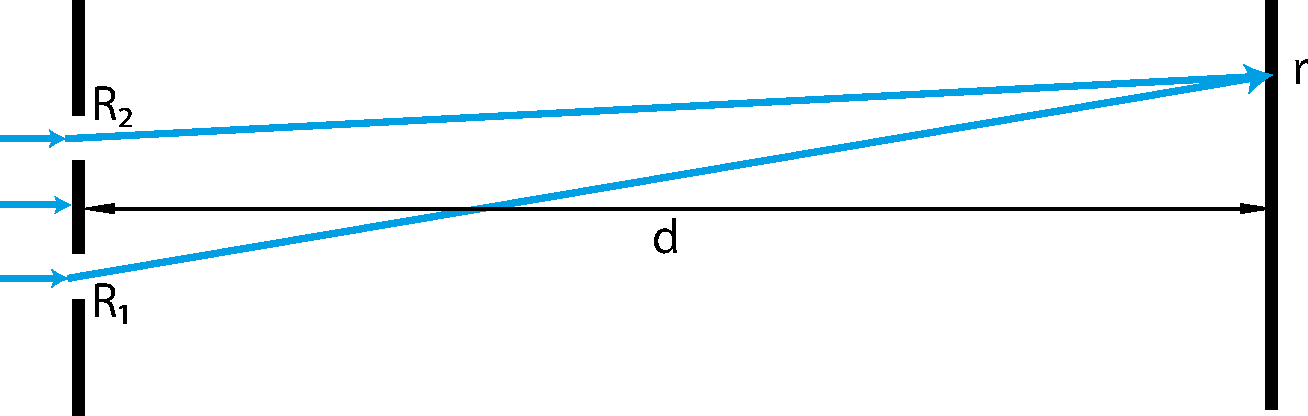
\includegraphics[width=0.8\linewidth]{images/doubleslit.pdf}
 	\caption{Schematic of double slit: Monochromatic light goes through slits located at $R_1$ and $R_2$. The intensity at a position $r$ on the scree (in distance $d$) is the superposition of both paths.  If the slits are within the lateral coherence area of the source, the visibility of the interference pattern depends on the path length difference in comparison to the coherence time $\tau$.}
 	 \label{fig:doubleslit}
 \end{figure}


\paragraph{First order coherence $g_1(t)$}

Definition of $g_1$
\begin{equation}
	g^{(1)}(\vec{r}_1,t_1;\vec{r}_2,t_2= \frac{\left< E^*(\vec{r}_1,t_1)E^*(\vec{r}_2,t_2)E(\vec{r}_1,t_1)E(\vec{r}_2,t_2) \right>}{\left<\left | E(\vec{r}_1,t_1)\right |^2 \right> \left< \left |E(\vec{r}_2,t_2)\right |^2 \right>}	
\end{equation}
\begin{equation}
V=\left|g_1\right|
\end{equation}

Int
-along Glauber/Statistical Optics Goodman




\paragraph{Second order coherence $g_2(t_1,t_2)$}
The definition of $g_1$ can be extended to the second order by
\begin{equation*}
	g^{(2)}(\vec{r}_1,t_1;\vec{r}_2,t_2= 
	\frac{\left< E^*(\vec{r}_1,t_1)E^*(\vec{r}_2,t_2)E(\vec{r}_1,t_1)E(\vec{r}_2,t_2) \right>}{\left<\left | E(\vec{r}_1,t_1)\right |^2 \right> \left< \left |E(\vec{r}_2,t_2)\right |^2 \right>}	
\end{equation*}
For classical fields normalized correlations of intensities:
\begin{equation}
	g^{(2)}(\vec{r}_1,t_1;\vec{r}_2,t_2)= 
		\frac{\left< I(\vec{r}_1,t_1)I(\vec{r}_2,t_2 \right>}{\left<I(\vec{r}_1,t_1)\right>\left<I(\vec{r}_1,t_1)\right>}	
\end{equation}

\paragraph{Van Cittert Zernicke}

%-Hanbury Brown and Twist
\section{Hanburry Brown Twiss}
Hanburry Brown and Twiss 


\paragraph{Siegert Relation for Pseudo-Thermal Light}

%-Single Photon Emitters/2nd Quant description
%(siehe Referenzen in Schaller/resonance fluorescence)
%-Fluorescence g2
%$2 Level with finite Lifetime -> Spectrum of fluorescence
\section{X-Ray Fluorescence}

\section{Intensity Correlations using X-Ray Fluorescence}
\section{Signal to Noise Considerations}
%- SNR
%will use Peak/stdev bg definition
Which factors influence SNR
-lifetime/pulsewidth
-polarisation
-sampling conditions / undersampling
-sample thickness / coherence length
-N images
-N photons
\label{chap:theory}

\section{Kossel Lines}

